\documentclass{beamer}

\def\Tiny{\fontsize{6pt}{6pt}\selectfont}
\def\supertiny{\fontsize{4pt}{4pt}\selectfont}

\mode<presentation>
{
  \usetheme{Warsaw}
  % \setbeamercovered{transparent}
  \usecolortheme{crane}
}


\usepackage{graphicx, ifthen, listings}

\usepackage[czech]{babel}
% \usefonttheme{professionalfonts}
\usepackage{times}
\usepackage{amsmath}
\usepackage[utf8]{inputenc}
\usepackage{wrapfig}

\usepackage[T1]{fontenc}

\lstset{ basicstyle=\tiny, stringstyle=\ttfamily, showstringspaces=false }

\everymath{\displaystyle}

\setbeamerfont{frametitle}{size=\large}
\setbeamerfont{subsection in toc}{size=\scriptsize}

\makeatletter\newenvironment{blackbox}{%
   \begin{lrbox}{\@tempboxa}\begin{minipage}{0.95\columnwidth}}{\end{minipage}\end{lrbox}%
   \colorbox{black}{\usebox{\@tempboxa}}
}\makeatother

\title[IMF (1)]{Informatika pro moderní fyziky (1)\\základy automatizace; jednoduché zpracování a vizualizace dat}

\author[Franti\v{s}ek HAVL\r{U}J, ORF ÚJV Řež]{Franti\v{s}ek HAVL\r{U}J\\{\scriptsize \emph{e-mail: haf@ujv.cz}}}

\date{zimní semestr 2026/2027 – 24. září 2026}

\institute[ORF ÚJV Řež]
{ÚJV Řež – oddělení Reaktorové fyziky a podpory palivového cyklu}

\AtBeginSection[]
{
\begin{frame}<beamer>
\frametitle{Obsah}
\tableofcontents[currentsection,hideothersubsections]
\end{frame}
}

\begin{document}

\begin{frame}
  \titlepage
\end{frame}

\begin{frame}
  \tableofcontents
\end{frame}

\section{Úvod}

\subsection{Sylabus semináře}

\begin{frame}{Profil absolventa předmětu}
  \begin{itemize}
    \item chápe počítač nikoli jako psací stroj anebo černou skříňku pro specializované aplikace, ale především jako flexibilní a vysoce univerzální nástroj pro každodenní úkoly ve zpracování dat, jejich prezentaci a tvorbě dokumentů
    \item orientuje se v~moderních paradigmatech praktické informatiky, programování na úrovni běžných skriptů je pro něj samozřejmostí a díky solidnímu přehledu je schopen se v~daném problému zorientovat a vybrat si pro jeho řešení vhodný nástroj
    \item není nucen vykonávat mechanickou a nudnou činnost, ale úkoly řeší kreativně - raději si ad hoc vytvoří na míru šitý skript, který jej ochrání před lidskou chybou i frustrací z~monotónnosti
  \end{itemize}
\end{frame}

\begin{frame}{Průběh výuky}
  \begin{itemize}
    \item zadání praktické úlohy, jejíž vyřešení je motivací pro obsah lekce
    \item přednáška na probírané téma, poskytující jak teoretický základ, tak přehled konkrétních nástrojů a postupů
    \item samostatná práce na řešení daného problému
    \item společná diskuse nad jednotlivými řešeními a jejich zhodnocení
  \end{itemize}
\end{frame}

\begin{frame}{Organizačně}
  \begin{itemize}
    \item čtvrtek 14:00-16:30 bez organizované přestávky (každý dle vlastních potřeb)
    \item předpokládá se aktivní účast (v uvozovkách povinná)
    \item v případě absence: vyžaduju po vás, abyste si \textbf{doplnili vše z lekce a měli hotové to, co ostatní} -- lekce na sebe většinou navazují!
    \item těm, kdo celý semestr chodili, zadám v posledním týdnu před Vánoci zápočtovou úlohu
  \end{itemize}
\end{frame}

\subsection{K čemu je počítač?}

\begin{frame}{K čemu je počítač?}
  \begin{columns}
    \column{0.6\textwidth}
    \begin{itemize}
      \item počítače udělají cokoliv, pokud na to existuje postup
      \item pokud na něco existuje postup, není na to potřeba člověk
      \item existuje-li postup, existuje také algoritmus
      \item kdo má algoritmus, může napsat program
    \end{itemize}
    \column{0.4\textwidth}
    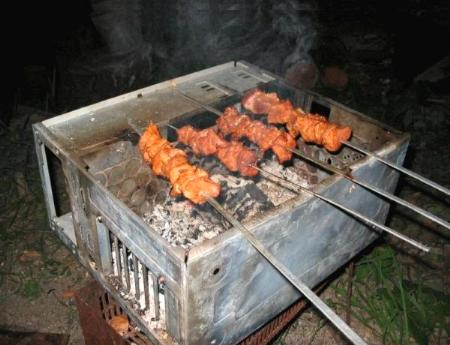
\includegraphics[width=\columnwidth]{computerbarbie}
  \end{columns}
\end{frame}

\begin{frame}{Proč se zabývat automatizací?}
  \begin{columns}
    \column{0.6\textwidth}
    \begin{itemize}
      \item mechanická práce je otravná
      \item program neudělá (náhodnou) chybu
      \item skript trvá stejně dlouho pro libovolný objem dat
      \item pokud je potřeba něco pozměnit nebo jen zpracování zopakovat, je ruční práce vepsí
    \end{itemize}
    \column{0.4\textwidth}
    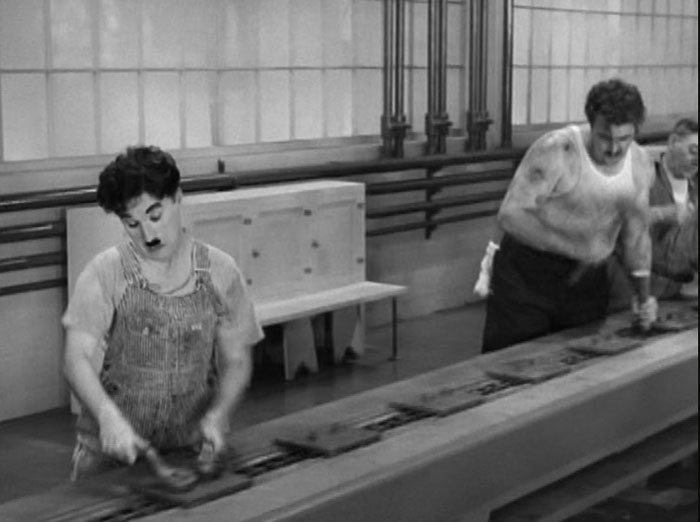
\includegraphics[width=\columnwidth]{chaplin}
  \end{columns}
\end{frame}

\begin{frame}{Má cenu se to učit v době AI?}
  \begin{itemize}
    \item zaprvé nevím 
    \item zadruhé já sám dělám aktuálně tak 90\% v Claude Code 
    \item zatřetí už jsem kvůli tomu zničil spoustu věcí
    \item začtvrté si myslím, že je stejně potřeba to umět, i když si to s AI hodně ulehčíme
  \end{itemize}
\end{frame}

\begin{frame}{Jak AI v tomto předmětu používat a nepoužívat -- návrh}
  \begin{itemize}
    \item ptejte se ho na co chcete
    \item nechte si poradit jak se má něco konkrétního udělat
    \item zkuste mu neposílat celý svůj kód, aby ho upravil
    \item nenechte si kód napsat
  \end{itemize}
\end{frame}

\subsection{Problém č. 1: vykreslování dat z~detektoru}

\begin{frame}{Zadání}
  \begin{block}{\# 1}
    Na konci provozní směny je potřeba vyhodnotit signály ze čtyř detektorů a vykreslit je do grafu (signál v~závislosti na čase). Data dostáváte v~jednoduchém textovém souboru (dva sloupce, spousta řádků). Je potřeba vykreslit do jednoho grafu všechny čtyři detektory. Potíž je, že taková data přicházejí každý den - tento úkol je tedy potřeba řešit opakovaně.
  \end{block}
  \begin{block}{S hvězdičkou}
    Počet detektorů je proměnný (1 až 9).
  \end{block}
\end{frame}

\begin{frame}{Příklad}
  \begin{center}
    
\includegraphics[width=0.6\columnwidth]{plot4}
  \end{center}
\end{frame}

\subsection{Problém č. 2: jehla v kupce sena}

\begin{frame}{Zadání}
  \begin{block}{\# 2}
    Adresář plný CSV souborů (stovky souborů) obsahuje data, která jsou záznamy signálů s lineární závislostí.

    V pěti z nich jsou ale poruchy - data ležící zcela mimo přímku.

    Kde?
  \end{block}
\end{frame}

\begin{frame}{Příklad - dobrý signál}
  \begin{center}
      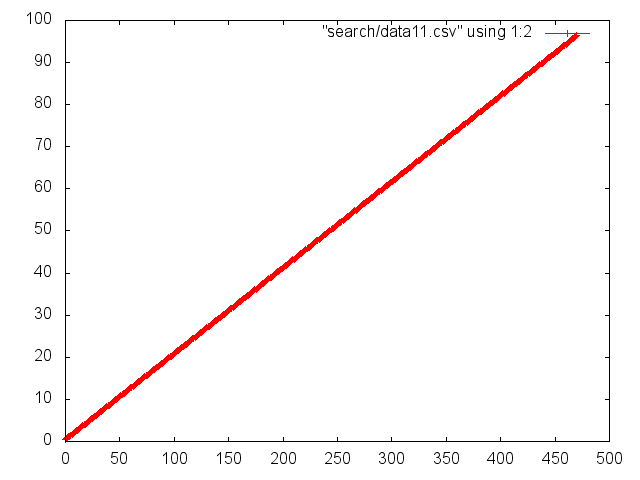
\includegraphics[width=0.6\columnwidth]{search_good}
      \end{center}
\end{frame}
\begin{frame}{Příklad - špatný signál}
  \begin{center}
      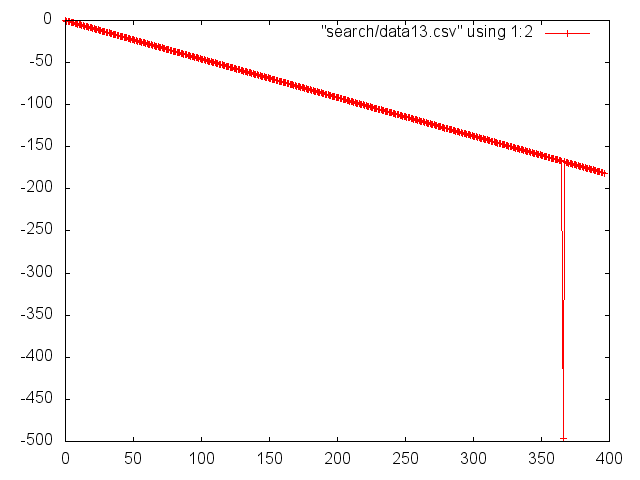
\includegraphics[width=0.6\columnwidth]{search_bad}
      \end{center}
\end{frame}


\subsection{Problém č. 3: zmatek v laborce}

\begin{frame}{Zadání}
  \begin{block}{\# 3}
    V jedné tabulce máme seznam vzorků půdy, jejich datum pořízení a místo odběru, v jiné změřenou aktivitu z laboratoře.

    To všechno musíme dostat dohromady a dopočítat se původní aktivity vzorků v době jejich odběru.

    Do toho je potřeba výsledky nějak dostat do excelu. Navíc bychom se možná rádi trochu předvedli a vzorky a jejich aktivity vykreslili do mapy.
  \end{block}
\end{frame}

\subsection{Problém č. 4: mnoho výpočtů, inženýrova smrt}

\begin{frame}{Zadání}
  \begin{block}{\# 4}
    Při přípravě základního kritického experimentu je pomocí MCNP potřeba najít kritickou polohu regulační tyče R2.

    Jak se tato poloha změní při změně polohy tyče R1?
  \end{block}
\end{frame}


\section{Odbočka: správa zdrojového kódu}

\begin{frame}{Jak mít uložený zdrojový kód}
  \begin{itemize}
    \item to, že mám na disku hromadu souborů a `jen tak' je edituju, přináší spoustu problémů
    \item pokud udělám chybu/něco se rozbije, nemám se jak vrátit, nemám přehled o průběhu změn
    \item pokud chci mít víc verzí najednou (stabilní / vývojová), nemám jak zajistit konzistenci
    \item není jak se vracet ke starším verzím, problémy de facto nelze reprodukovat
  \end{itemize}
\end{frame}

\begin{frame}{Práce v týmu}
  \begin{itemize}
    \item pokud na projektu pracuje víc lidí, stává se z problému noční můra
    \item jak dát dohromady změny od více lidí?
    \item jak zajistit, že všichni používají stejnou verzi?
    \item pro dokumenty už jsou různá více či méně dobrá řešení (slučování změn v MS Office, online nástroje jako Google Documents)
  \end{itemize}
\end{frame}

\begin{frame}{Jaké jsou možnosti}
  \begin{itemize}
    \item nabízí se schovávat si každý týden verzi a pokusit se v tom udržet pořádek
    \item dbát na správná jména složek/souborů
    \item za žádnou cenu nemodifikovat verzovanou složku (read-only...)
    \item vést záznam o změnách, všechno podrobně dokumentovat
  \end{itemize}
\end{frame}

\begin{frame}{Jak se to dělá správně}
  \begin{itemize}
    \item existují takzvané version control systems -- VCS, které se o řešení tohoto problému postarají za nás
    \item základní princip: neukládám aktuální verze souborů, ale pouze \emph{změny}
    \item k čemu to je -- změny je možné mezi sebou \textbf{sčítat}, což je (po lehkém zamyšlení) naprosto geniální a řeší to všechno
    \item pokud mám paralelní změny (dva různí lidé něco změní), není to obvykle vůbec žádný problém, pokud nezměnili stejné místo
    \item můžu rekonstruovat libovolný bod v historii
  \end{itemize}
\end{frame}

\begin{frame}{Řešení konfliktů -- merging}
  \begin{itemize}
    \item pokud dva uživatelé udělají změnu zároveň, co se stane?
    \item když konflikt nenastal na stejném řádku stejného souboru, tak je to v pořádku
    \item v opačném případě to prostě musí vyřešit uživatel ručně (ale není to častá situace)
    \item spojení změn se ale vždycky musí dělat lokálně (na straně uživatele), aby se zamezilo sémantickému konfliktu
  \end{itemize}
\end{frame}

\begin{frame}{Paralelní větve -- branches}
  \begin{itemize}
    \item často se hodí mít víc verzí najednou
    \item jednak různé stupně experimentálnosti (stabilní, testovací, vývojová)
    \item jednak pokud chci přidat větší feature, tak to nechci míchat s hlavní větví vývoje
    \item VCS to většinou umí řešit -- strom vývoje nemusí být lineární, ale může se větvit
  \end{itemize}
\end{frame}

\begin{frame}{Přehled VCS}
  \begin{itemize}
    \item CVS -- první standardní VCS, dnes již zcela překonaný
    \item SVN -- moderní centralizovaný VCS, donedávna nejpoužívanější řešení
    \item Git -- dnešní de facto standard, pokročilý distribuovaný VCS s geniální podporou branches
    \item Mercurial, Bazaar -- méně obvyklé alternativy Gitu
  \end{itemize}
\end{frame}

\begin{frame}{Centralizovaný vs. distribuovaný VCS}
  \begin{itemize}
    \item centralizovaný: mám jeden centrální repozitář, do kterého ukládají změny všichni uživatelé
    \item distribuovaný: každý uživatel má celý repozitář u sebe
    \item výhody -- lokální commity (bez spojení se serverem!), lokální branche, bezpečnost (vysoká redundance)
    \item nevýhody -- někomu to dělá problém pochopit a přijmout
  \end{itemize}
\end{frame}

\begin{frame}{Kdy je dobré používat VCS}
  \begin{itemize}
    \item vlastně vždycky, pokud pracuju s plaintextovými soubory (tj. zejména zdrojové kódy, skripty)
    \item využití pro binární data (což se týká de facto i wordovského dokumentu...) je velice omezené
    \item -- další důvod používat LaTeX! tam je samozřejmě všechno v pořádku
    \item výhody verzování (oproti tomu to ``jen někde mít'') jsou nedozírné
    \item za sebe můžu říct, že asi úplně všechnu svoji práci mám v nějakém repo
    \item a pro tu AI práci je to vlastně dneska úplně nezbytnost
  \end{itemize}
\end{frame}

\begin{frame}{Ukázka a příklad veřejných repozitářů}
  \begin{itemize}
    \item \texttt{http://github.com}
    \item \texttt{https://github.com/weshatheleopard/rubyXL}
    \item vhodné zejména pro open source projekty, ale umožňuje i soukromé repo
    \item velmi hezké GUI (přehledy změn, grafy větvení, issue tracker, komunikace mezi vývojáři)
    \item samozřejmě není problém si nainstalovat repozitář (např. \texttt{gitolite}) někde u sebe na serveru
  \end{itemize}
\end{frame}

\begin{frame}{Repozitář IMF}
  \begin{itemize}
    \item přejděte na \texttt{https://support.orf.ujv.cz/imf} -- to by mělo jít bez registrace
    \item v projektu \textbf{IMF 2026-2027} byste měli vidět vše pro dnešní den 
    \item nainstalujte si git https://git-scm.com/install/windows
    \item stáhněte si repozitář: \texttt{git clone https://support.orf.ujv.cz/imf/imf-2026-2027.git}
  \end{itemize}
\end{frame}

\begin{frame}{Váš vlastní repozitář}
  \begin{itemize}
    \item na našem ÚJV gitlabu se zaregistrujte
    \item vytvořte si prázdný repozitář a vyklonujte si ho
    \item a tam pracujte
  \end{itemize}
\end{frame}

\section{Ruční a poloautomatická řešení}

\subsection{Problém č. 1: rozbor situace}

\begin{frame}[fragile]{Vstupní data}
  \begin{columns}
    \column{0.7\textwidth}
      {\scriptsize
      \begin{verbatim}
0.00000e+00 0.00000e+00
1.00000e-04 1.01447e-03
2.00000e-04 4.62446e-04
3.00000e-04 6.92465e-04
4.00000e-04 4.48142e-03
5.00000e-04 6.95896e-03
6.00000e-04 5.12501e-03
7.00000e-04 2.62076e-03
...
      \end{verbatim}
      }
    \column{0.29\textwidth}
      \begin{block}{Formát CSV}
        $\bullet$ comma separated values

        $\bullet$ zobecnělo ale jako libovolný formát po sloupcích uložených dat

        $\bullet$ dobře se zpracovává, importuje do Excelu atd.
      \end{block}
  \end{columns}
\end{frame}

\begin{frame}{Klasické řešení (MS Excel)}
  \begin{itemize}
    \item jaké všechny kroky by bylo potřeba udělat?
    \item na který z~provedených kroků byl potřeba člověk -- co z~toho by nemohl stejně dobře udělat počítač sám?
    \item jaké jsou výhody a nevýhody ručního řešení?
  \end{itemize}
\end{frame}

\begin{frame}{Co by takové automatické řešení mohlo umět?}
  \begin{itemize}
    \item načte z daného adresáře soubory se záznamy
    \item vykreslí graf a uloží ho do souboru
    \item soubor jednoznačně pojmenuje a zkopíruje na vhodné místo
    \item uživatel by neměl v ideálním případě dělat vůbec nic
  \end{itemize}
\end{frame}

\begin{frame}{Komponenty pro automatizaci}
  \begin{block}{Funkční části}
    výkonné programy (např. kreslení grafů, generování tabulek/reportů, spouštění výpočtů) -- předpokladem je možnost spouštět program v~neinteraktivním (dávkovém) režimu
  \end{block}
  \pause
  \begin{block}{Jak to slepit dohromady}
    dávkový soubor (BAT) nebo skript -- je nutno vždy vhodně volit použité prostředky ve vztahu k~jednoduchosti, požadavkům na funkce, přenositelnosti
  \end{block}
\end{frame}

\begin{frame}{Jak postupovat s~automatickým řešením?}
  \begin{enumerate}
    \item vykreslit graf s~jedním detektorem
    \pause
    \item se všemi detektory
    \pause
    \item z~příkazové řádky
    \pause
    \item z~batch souboru
    \pause
    \item se jménem adresáře jako parametrem
  \end{enumerate}
\end{frame}

\begin{frame}{Gnuplot}
  \begin{columns}
    \column{0.7\textwidth}
      \begin{itemize}
        \item interaktivní i dávkový režim -- ideální pro automatizaci
        \item slušně konfigurovatelné 2D i 3D grafy
        \item i bez nastavení funguje velmi přijatelně
        \item široká paleta výstupních formátů
      \end{itemize}
    \column{0.29\textwidth}
      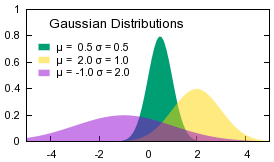
\includegraphics[width=\columnwidth]{gnuplot1}

      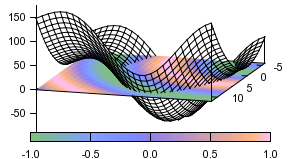
\includegraphics[width=\columnwidth]{gnuplot2}
  \end{columns}
\end{frame}

\subsection{Řešení}

\begin{frame}[fragile]{Vykreslení jednoho grafu v~gnuplotu}
  \begin{verbatim}
    gnuplot> plot "data1.csv"
  \end{verbatim}
  \pause
  \begin{center}
    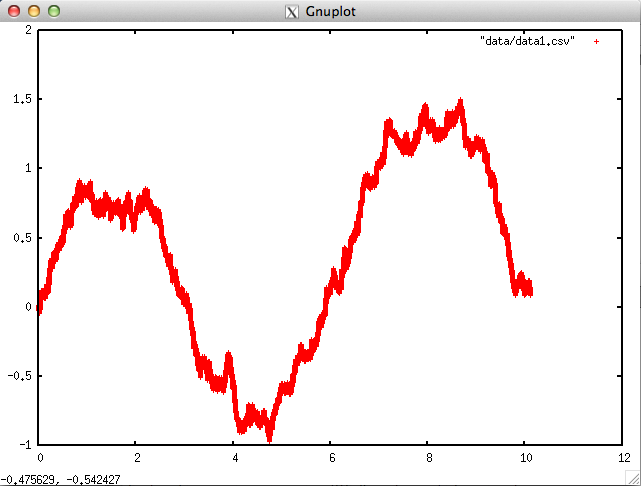
\includegraphics[width=0.6\textwidth]{gnuplot_interactive}
  \end{center}
\end{frame}

\begin{frame}[fragile]{Vykreslení všech grafů v~gnuplotu}
  \begin{verbatim}
    gnuplot> plot "data1.csv", "data2.csv", \
                  "data3.csv", "data4.csv"
  \end{verbatim}
  \pause
  \begin{center}
    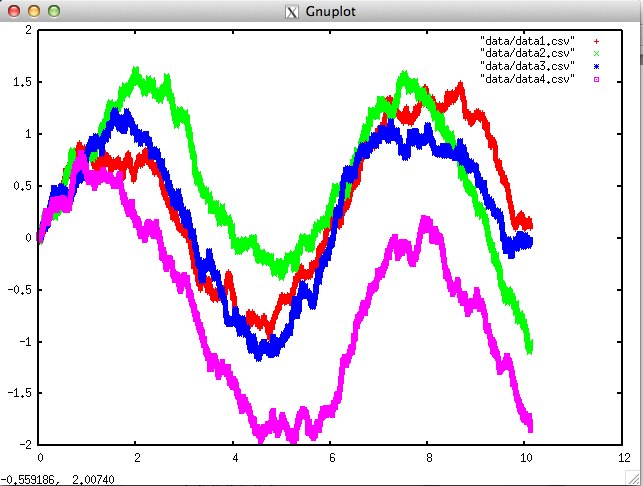
\includegraphics[width=0.6\textwidth]{gnuplot_interactive_all}
  \end{center}
\end{frame}

\begin{frame}[fragile]{Dávkové použití}
  \scriptsize
  \begin{verbatim}
    set terminal png
    set output "plot4.png"
    plot "gnuplot/data1.csv", "gnuplot/data2.csv", \
         "gnuplot/data3.csv", "gnuplot/data4.csv"
  \end{verbatim}
  \pause
  \begin{center}
    
\includegraphics[width=0.6\textwidth]{../gnuplot/plot4}
  \end{center}
\end{frame}

\begin{frame}[fragile]{BAT soubor (Windows)}
  Je pracné pokaždé vypisovat parametry na příkazovou řádku. .BAT soubory ve Windows fungují jednoduše, prostě se do nich dá psát jako do terminálu a připravit si tak jednodušší skript.
  {\scriptsize
  \begin{verbatim}
    "C:/Program Files/Gnuplot/bin/gnuplot.exe" plot.gp
  \end{verbatim}
  }
  (pozor na uvozovky kvůli mezeře v cestě. Cestu upravte podle skutečnosti na svém počítači.)
\end{frame}

\begin{frame}[fragile]{Shell skript (MacOS, Linux)}
  Skript bude trochu jednodušší a velmi podobný:
  \begin{verbatim}
    gnuplot plot.gp
  \end{verbatim}
  Uložte ho (konvence) s koncovkou \texttt{.sh}. Pozor, ještě je nutno jej změnit na spustitelný pomocí \texttt{chmod}, tedy pokud se jmenuje \texttt{plot.sh}, použijte:
  \begin{verbatim}
    chmod +x plot.sh
  \end{verbatim}
  -- to stačí udělat jednou, pak ho můžete libovolně editovat. Skript se pak z terminálu spustí:
  \begin{verbatim}
    ./plot.sh
  \end{verbatim}
\end{frame}

\begin{frame}[fragile]{BAT soubor s~parametrem}
  
  Co takhle adresář pro každý den? Vizte adresář `multidata'. Nemá smysl pokaždé ručně kopírovat vstup pro gnuplot a tak dále... 

  Stačí vědět, že BAT soubor může mít na příkazové řádce parametry. První parametr je uložen do proměnné \texttt{\%1} a to se nám bude hodit.

{\scriptsize
  \begin{verbatim}
    cd %1
    "C:/Program Files/Gnuplot/bin/gnuplot.exe" ../plot.gp
    cd ..
  \end{verbatim}
  }
\end{frame}

\begin{frame}[fragile]{Opět alternativa pro shell skript}
  Proměnné se označují místo procenta dolarem, tj. \texttt{\$1}:

  \begin{verbatim}
    cd $1
    gnuplot ../plot.gp
    cd ..
  \end{verbatim}
\end{frame}

\begin{frame}[fragile]{BAT soubor s~parametrem - vylepšení}
  Pokud si budeme chtít prohlédnout grafy, bude nutné vždy vlézt do adresáře a otevřít \texttt{plot.png}. Jde to ovšem vylepšit pomocí jednoduchého triku:
{\scriptsize
  \begin{verbatim}
    cd %1
    "C:/Program Files/Gnuplot/bin/gnuplot.exe" ../plot.gp
    copy plot.png ..\%1.png
    cd ..
  \end{verbatim}
  }
\end{frame}

\begin{frame}[fragile]{Totéž v shellu}
  \begin{verbatim}
    cd $1
    gnuplot ../plot.gp
    cp plot.png ../$1.png
    cd ..
  \end{verbatim}
\end{frame}

\subsection{Zhodnocení}

\begin{frame}{Jak moc jsme si pomohli?}
  \begin{itemize}
    \item jeden skript místo excelovské anabáze
    \item máme znovupoužitelný nástroj -- můžeme proces kdykoliv zopakovat
    \item nelze udělat žádnou ``ruční chybu''
    \item skript můžeme dát kolegovi a ten má práci hotovou úplně zadarmo
    \item skript lze periodicky spouštět bez účasti uživatele, možnost např. zobrazovat na intranetu aktuální grafy atd.
  \end{itemize}
\end{frame}

\subsection{Problém č. 2, 3, 4: jak na to?}

\begin{frame}{Stačí nám to na řešení problému č. 2, 3 a 4?}
  Zatím nevíme, jak:
  \begin{itemize}
    \item prohledat adresář a vygenerovat spoustu grafů
  \end{itemize}
  \begin{itemize}
    \item vygenerovat vstupní soubory pro MCNP
    \item spustit hromadu MCNP výpočtů
    \item vytahat výsledky z~MCNP výstupního souboru
  \end{itemize}
  \begin{itemize}
    \item propojovat data z více tabulek (i když se to dá v excelu naučit)
    \item získávat a vykreslovat geografická data
  \end{itemize}
  Budeme potřebovat nějaký těžší kalibr.
\end{frame}

\section{Skriptovací jazyky}

\subsection{Úvod do skriptování}

\begin{frame}{``klasické'' programování -- Pascal, C++}
  \begin{itemize}
    \item napsat zdroják, zkompilovat, slinkovat ...
    \item ... muset řešit binárku, která někde funguje a někde ne ...
    \item ... moc práce!
    \item (i když výhody jsou zřejmé -- rychlost, distribuce binárek místo zdrojáků, ``uzavřené'' prostředí)
    \item bylo by lepší mít někdy místo motorové pily sekeru
  \end{itemize}
\end{frame}

\begin{frame}{Interpretované jazyky / skripty}
  \begin{itemize}
    \item textový vstupní soubor (zdrojový kód) + interpret
    \item vhodné pro aplikace bez vysokých nároků na systém
    \item nebo tam, kde je zásadní snížit nároky na vývoj
    \item tj. ideální pro jednoúčelové a krátkodobě žijící programy
    \item většinou ``volnější'' pojetí programování, z~čehož plyne například řádově elegantnější práce s~textem
  \end{itemize}
\end{frame}

\begin{frame}{Vlastnosti skriptovacích jazyků}
  \begin{block}{Výhody}
    \begin{itemize}
      \item dokonalá přenositelnost (textové vstupní soubory)
      \item nic se nekompiluje
      \item většinou syntakticky úsporné
    \end{itemize}
  \end{block}
  \pause
  \begin{block}{Nevýhody}
    \begin{itemize}
      \item zdrojový kód je otevřený (ne vždy se to hodí)
      \item pomalé a paměťově náročné
      \item bez kontroly správnosti při kompilaci
    \end{itemize}
  \end{block}
\end{frame}

\begin{frame}{Přehled hlavních jazyků}
  \begin{description}
    \item[BAT] -- vhodné pouze pro to nejjednodušší použití; i když jsou k~mání některé trochu složitější funkce, jejich použití je hodně neobratné a neefektivní
    \item[BASH] -- podstatně mocnější alternativa BAT souborů v~prostředí Unixu; nepříliš intuitivní syntaxe a absence náročnějších operací
    \item[Perl] -- kompaktní a efektní jazyk, který je všude nainstalovaný, ale nedá se (vůbec) číst a už i pole apod. jsou nekřesťansky obskurní
    \item[Python] -- velmi slušný jazyk, který snese i ``vážnější'' využití, ale za cenu trochu vyšší obtížnosti
    \item[Ruby] -- elixír síly a zázračná pilulka: intuitivní, snadný, všemocný, rozšířený a k~tomu ryze objektový
  \end{description}
\end{frame}

\subsection{Úvod do jazyka Ruby}

\begin{frame}{Jazyk Ruby}
  \begin{itemize}
    \item čistě objektový interpretovaný jazyk
    \item interprety existují pro širokou škálu platforem
    \item velmi elegantní syntaxe
    \item nevýhodou je stále ještě relativní pomalost
    \item aktuální verze 4.0 (rozumné minimum je 3.4, míň nebrat)
  \end{itemize}
\end{frame}

\begin{frame}[fragile]{Ukázka Ruby (1)}
  Každý programátor tím začíná ...
  \begin{block}{}
    \smallskip \footnotesize
    {\scriptsize \begin{verbatim}
      puts "Hello world!"
    \end{verbatim}}
  \end{block}
  \pause
  \begin{block}{}
    \smallskip \footnotesize
    {\scriptsize \begin{verbatim}
      Hello world!
    \end{verbatim}}
  \end{block}
\end{frame}

\begin{frame}[fragile]{Ukázka Ruby (2)}
  Proměnné, \texttt{print} vs. \texttt{puts}, aritmetika
  \begin{block}{}
    \smallskip \footnotesize
    {\scriptsize \begin{verbatim}
      a = 4
      b = 5
      print "4 + 5 = "
      puts a + b
    \end{verbatim}}
  \end{block}
  \pause
  \begin{block}{}
    \smallskip \footnotesize
    {\scriptsize \begin{verbatim}
      4 + 5 = 9
    \end{verbatim}}
  \end{block}
\end{frame}

\begin{frame}[fragile]{Ukázka Ruby (3)}
  In-line výrazy v~řetězcích
  \begin{block}{}
    \smallskip \footnotesize
    {\scriptsize \begin{verbatim}
      a = 4
      b = 5
      puts "#{a} + #{b} = #{a+b}"
    \end{verbatim}}
  \end{block}
  \pause
  \begin{block}{}
    \smallskip \footnotesize
    {\scriptsize \begin{verbatim}
      4 + 5 = 9
    \end{verbatim}}
  \end{block}
\end{frame}

\begin{frame}[fragile]{Důležitá vsuvka}
  Řetězec
  \begin{block}{}
    \smallskip \footnotesize
    {\scriptsize \begin{verbatim}
      "a"
    \end{verbatim}}
  \end{block}
  \pause
  Proměnná
  \begin{block}{}
    \smallskip \footnotesize
    {\scriptsize \begin{verbatim}
      a
    \end{verbatim}}
  \end{block}
  \pause
  Řetězec s proměnnou uvnitř
  \begin{block}{}
    \smallskip \footnotesize
    {\scriptsize \begin{verbatim}
      "#{a}"
    \end{verbatim}}
  \end{block}
\end{frame}

\begin{frame}[fragile]{Ukázka Ruby (4)}
  Rozsahy a cykly
  \begin{block}{}
    \smallskip \footnotesize
    {\scriptsize \begin{verbatim}
      (1..5).each do |i|
        puts "#{i} * #{i} = #{i * i}"
      end
    \end{verbatim}}
  \end{block}
  \pause
  \begin{block}{}
    \smallskip \footnotesize
    {\scriptsize \begin{verbatim}
      1 * 1 = 1
      2 * 2 = 4
      3 * 3 = 9
      4 * 4 = 16
      5 * 5 = 25
    \end{verbatim}}
  \end{block}
\end{frame}


\begin{frame}[fragile]{Ukázka Ruby (5)}
  Pětkrát nic umořilo osla (opakování, ne cyklus)
  \begin{block}{}
    \smallskip \footnotesize
    {\scriptsize \begin{verbatim}
      5.times do
        puts "nic"
      end
    \end{verbatim}}
  \end{block}
  \pause
  \begin{block}{}
    \smallskip \footnotesize
    {\scriptsize \begin{verbatim}
      nic
      nic
      nic
      nic
      nic
    \end{verbatim}}
  \end{block}
\end{frame}

\subsection{První kroky s~Ruby}

\begin{frame}[fragile]{IRb}
  Pro první ozkoušení (a i pro některé úkoly v~praktickém životě) se hodí ``příkazová řádka'' Ruby, tzv. \textbf{Interactive Ruby} (\texttt{IRb}):
  \pause
  \begin{block}{}
    {\scriptsize \begin{verbatim}
      irb(main):001 > 2+2
       => 4
      irb(main):002 > a = 5
       => 5
      irb(main):003 > b = 6
       => 6
      irb(main):004 > a * b
       => 30
    \end{verbatim}}
  \end{block}

\end{frame}

\begin{frame}[fragile]{Proměnné, výpis na terminál}
  V Ruby (jak je u skriptů zvykem) se proměnné nedeklarují:
  \begin{block}{}
    {\scriptsize \begin{verbatim}
      a = 5
      a = a * a
      long_string = "looooong string"
    \end{verbatim}}
  \end{block}
  \pause
  Výpis se děje pomocí print, resp. puts (bez/s~koncem řádku); \texttt{\#\{...\}} vkládá do řetězce libovolný výraz:
  \begin{block}{}
    {\scriptsize \begin{verbatim}
      print a
      puts "a = #{a}"
    \end{verbatim}}
  \end{block}
\end{frame}

\begin{frame}[fragile]{Pole a hashe}
  Pole je seznam:
  \begin{block}{}
    {\scriptsize \begin{verbatim}
      a = []
      a << 5
      a += [6]
      puts a.size
    \end{verbatim}}
  \end{block}
  \pause
  Hash, neboli slovník či asociativní pole:
  \begin{block}{}
    {\scriptsize \begin{verbatim}
      b = {}
      b[3] = 7
      b["foo"] = "bar"
    \end{verbatim}}
  \end{block}
\end{frame}

\begin{frame}[fragile]{Rozsahy a cykly}
  Rozsahy (ranges) - se dvěma tečkami včetně posledního elementu, se třemi bez něj
  \begin{block}{}
    {\scriptsize \begin{verbatim}
      a = (1..5)
      b = (1...5)
      puts "yay!" if a.size == b.size + 1
    \end{verbatim}}
  \end{block}
  \pause
  Ruby nepoužívá klasický cyklus, ale iterátor (přes téměř cokoliv):
  \begin{block}{}
    {\scriptsize \begin{verbatim}
      (1..5).each do |i|
        puts i * i
      end
      b = {}; b["key1"] = 6; b["key2"] = 8
      b.each do |key, value|
        puts "#{key} => #{value}"
      end
    \end{verbatim}}
  \end{block}
\end{frame}

\begin{frame}[fragile]{Práce s~řetězci, include, split, sub}
  Řetězce v~Ruby jsou neomezené délky (pár mega se tam určitě vejde) a dá se s~nimi provádět ledacos.
  \begin{block}{}
    {\scriptsize \begin{verbatim}
      s = "lazy dog"
      if s.include?("lazy")
        puts "lazy!!!"
      end
    \end{verbatim}}
  \end{block}
  \pause
  Rozdělit? Nahradit?
  \begin{block}{}
    {\scriptsize \begin{verbatim}
      puts s.sub("lazy", "crazy")
      a = s.split
      puts "#{a[1]} #{a[0]}"
    \end{verbatim}}
  \end{block}
\end{frame}

\begin{frame}[fragile]{Načítání a zápis do souboru}
  Soubor a terminál, to je vlastně jedno:
  \begin{block}{}
    {\scriptsize \begin{verbatim}
      File.open("animals.txt", "w") do |f|
        f.puts "quick brown fox"
      end
    \end{verbatim}}
  \end{block}
  \pause
  Nejjednodušší čtení je po řádcích:
  \begin{block}{}
    {\scriptsize \begin{verbatim}
      IO.foreach("data.csv") do |line|
        ...
      end
    \end{verbatim}}
  \end{block}
\end{frame}

\begin{frame}[fragile]{Práce s~adresářem}
  Jak projít všechny soubory v~adresáři? V Pascalu utrpení, v~Ruby iterátor:
  \begin{block}{}
    {\scriptsize \begin{verbatim}
      Dir["*"].each do |filename|
        puts filename
      end
    \end{verbatim}}
  \end{block}
  \pause
  Lze použít podle očekávání libovolnou masku nebo cestu:
  \begin{block}{}
    {\scriptsize \begin{verbatim}
      Dir["data/*.csv"].each do |filename|
        IO.foreach(filename) do |line|
          puts line
        end
      end
    \end{verbatim}}
  \end{block}
\end{frame}

\begin{frame}{A to je vše, přátelé!}
  \begin{center}
    
\includegraphics[width=0.7\textwidth]{looney_tunes}
  \end{center}
\end{frame}

\end{document}
